\subsubsection{Gut microbiota recovery after auto-FMT}

Allogeneic haematopoietic stem-cell transplantation (allo-HSCT) exposes the
intestinal microbiota to conditioning therapy and intensive antibiotic
treatment. This perturbation can deplete obligate anaerobes and alpha diversity,
permit domination by individual taxa and increase the risk of bloodstream
infection and mortality \cite{taur2012domination,shono2016antibiotics,
peled2020microbiota}. To examine microbiota restoration after this strong
ecological disturbance, we reanalysed longitudinal 16S rRNA gene profiles from
the single-centre, open-label randomized trial of autologous faecal microbiota
transplantation (auto-FMT; NCT02269150) reported by Taur et al.
\cite{taur2018reconstitution}. Participants banked a pathogen-screened,
adequately diverse stool sample before allo-HSCT. After neutrophil engraftment,
patients with quantitative-PCR evidence of marked Bacteroidetes depletion were
randomized 1:1 to receive their own stored microbiota by retention enema or no
FMT. The published microbiome cohort comprised the first 25 evaluable
participants among 31 randomized patients: 14 auto-FMT recipients and 11
controls. Evaluable participants had both a pre-randomization stool and a stool
collected within 14 days after randomization \cite{taur2018reconstitution}.

The original trial showed that auto-FMT increased inverse-Simpson diversity and
returned community composition towards its pre-HSCT state
\cite{taur2018reconstitution}. Here we asked a more specific ecological
question: did auto-FMT advance recovery towards each patient's own pre-HSCT
community, beyond differences in baseline diversity and the spontaneous
time-dependent recovery that follows allo-HSCT? We used the earliest observed
pre-HSCT sample as the personal reference and represented alpha, beta and gamma
diversity, together with distance from that reference, in the same HRIC
coordinate system. Figure~\ref{fig:fmt-individual} uses the clinical calendar,
on which day 0 is the allo-HSCT infusion. For the randomized comparison
(Fig.~\ref{fig:fmt-randomized}), event day 0 is auto-FMT in the treatment arm
and randomization in the control arm. The primary recovery window was event
days 1--30; index-day stools were excluded because their collection order
relative to auto-FMT was unavailable.

We first resolved recovery at the level of individual patients
(Fig.~\ref{fig:fmt-individual}). The two displayed patients were selected as
descriptive examples of contrasting trajectories and were not used to estimate
the treatment effect. In patient 0028, alpha diversity fell to 0.0083 three
days before auto-FMT and was 0.0467 two days before auto-FMT, compared with a
personal pre-HSCT value of 0.0630. It increased to approximately 0.066 one day
after auto-FMT and remained above the operational 80\% recovery threshold at
the next observed sampling day. Phase-level gamma diversity increased from
0.027 before auto-FMT to 0.083 afterwards. By contrast, patient 0009, assigned
to control, remained below a personal pre-HSCT alpha diversity of 0.116 after
randomization and did not show sustained 80\% recovery within 60 days.

The taxon-resolved trajectories linked these diversity changes to community
reorganization. Bacteroidetes relative abundance is shown to provide the
eligibility context, although the trial threshold was measured by quantitative
PCR and is not numerically interchangeable with the plotted 16S relative
abundance \cite{taur2018reconstitution}. The alluvial decomposition assigns the
complete alpha deficit, $1-\alpha$, to taxa in each sample. In patient 0028,
the dominant pre-index contribution from Listeriaceae contracted after
auto-FMT as the deficit became distributed across a broader set of taxa.
Patient 0009 instead passed through several domination patterns without
returning to the personal alpha benchmark. These contributions describe the
taxonomic structure of diversity loss and recovery; they are neither relative
abundances nor differential-abundance tests.

At the arm level, the clearest early difference was recovery of personal
community composition (Fig.~\ref{fig:fmt-randomized}). After adjustment for
personal pre-HSCT alpha diversity, the nearest pre-index distance and
randomization day, mean HRIC-coordinate distance from the personal baseline
over days 1--30 was 0.496 units lower with auto-FMT than with control (95\%
stratified patient-bootstrap interval, $-0.617$ to $-0.230$;
$P=4.0\times10^{-4}$; 4,999 resamples). The adjusted difference was $-0.471$
at day 14 and $-0.349$ at day 30, but narrowed to $-0.119$ by day 60 (95\%
model-based CI, $-0.554$ to $+0.316$). Auto-FMT therefore shifted communities
towards their own pre-HSCT state during the first month, whereas later
spontaneous recovery reduced the separation between arms.

Alpha diversity changed in the same direction, but with greater patient-level
uncertainty. The adjusted auto-FMT minus control difference averaged over days
1--30 was $+0.0235$ (95\% stratified patient-bootstrap interval, $-0.0015$ to
$+0.0373$; $P=0.0668$). Model-based point contrasts were $+0.0219$ at day 14
and $+0.0136$ at day 30, but $-0.0018$ at day 60. Moreover, the
treatment-by-time slope interactions were not supported during either days
1--14 ($P=0.208$) or days 15--60 ($P=0.147$). Thus, the data indicate an early
shift to a more recovered state, most clearly for personal composition, rather
than a continuously steeper alpha-diversity trajectory throughout follow-up.

Sensitivity analyses addressed baseline imbalance and pre-index dynamics. The
between-arm difference in pre-index alpha slope did not reach the conventional
significance threshold ($P=0.058$), and there was no evidence of a corresponding
difference in distance to baseline ($P=0.373$). An event-time
difference-in-differences analysis, which subtracted the adjusted arm
difference at day $-1$, retained an early auto-FMT advantage for alpha
diversity ($+0.0580$; 95\% model-based CI, $+0.0350$ to $+0.0809$) and distance
to baseline ($-0.603$; $-0.858$ to $-0.348$). A complementary threshold
analysis yielded the same direction: among patients below 80\% of personal
baseline at the index day, 6 of 13 auto-FMT recipients and 1 of 8 controls had
a crossing confirmed at the next observed sample by day 30. This sparse,
irregularly sampled comparison was not significant (two-sided Fisher's exact
$P=0.174$) and is descriptive.

Finally, the coordinate decomposition identified taxa associated with alpha
recovery. In the early auto-FMT window, the largest reductions in the alpha
deficit were assigned to Listeriaceae and Enterobacteriaceae, followed by
smaller contributions from Lactococcus, Streptococcus and Lactobacillus.
Control patients shared part of this profile, but concordance between arms was
moderate among the union of their 50 largest absolute contributors (Spearman
$\rho=0.58$ in the early window and 0.49 later). Only five taxa were shared
between the arm-specific top-10 sets at either landmark. Recovery therefore
reflected a partly shared, partly patient- and arm-specific rebalancing rather
than the behaviour of a single universal taxon.

Together, these analyses indicate that auto-FMT was associated with earlier
restoration towards each patient's pre-HSCT gut community in the evaluable
randomized microbiome cohort. Support was strongest for compositional
restoration and directionally consistent, but less precise, for alpha
diversity. The attenuation of both contrasts by day 60 is more consistent with
shortening the period of severe microbiota disruption than with producing a
persistent diversity advantage. This inference is restricted to microbiota
recovery in evaluable participants; it does not establish effects on infection,
graft-versus-host disease, mortality or other clinical outcomes, and it is not
an intention-to-treat analysis of all randomized patients.

\begin{figure*}[t]
  \centering
  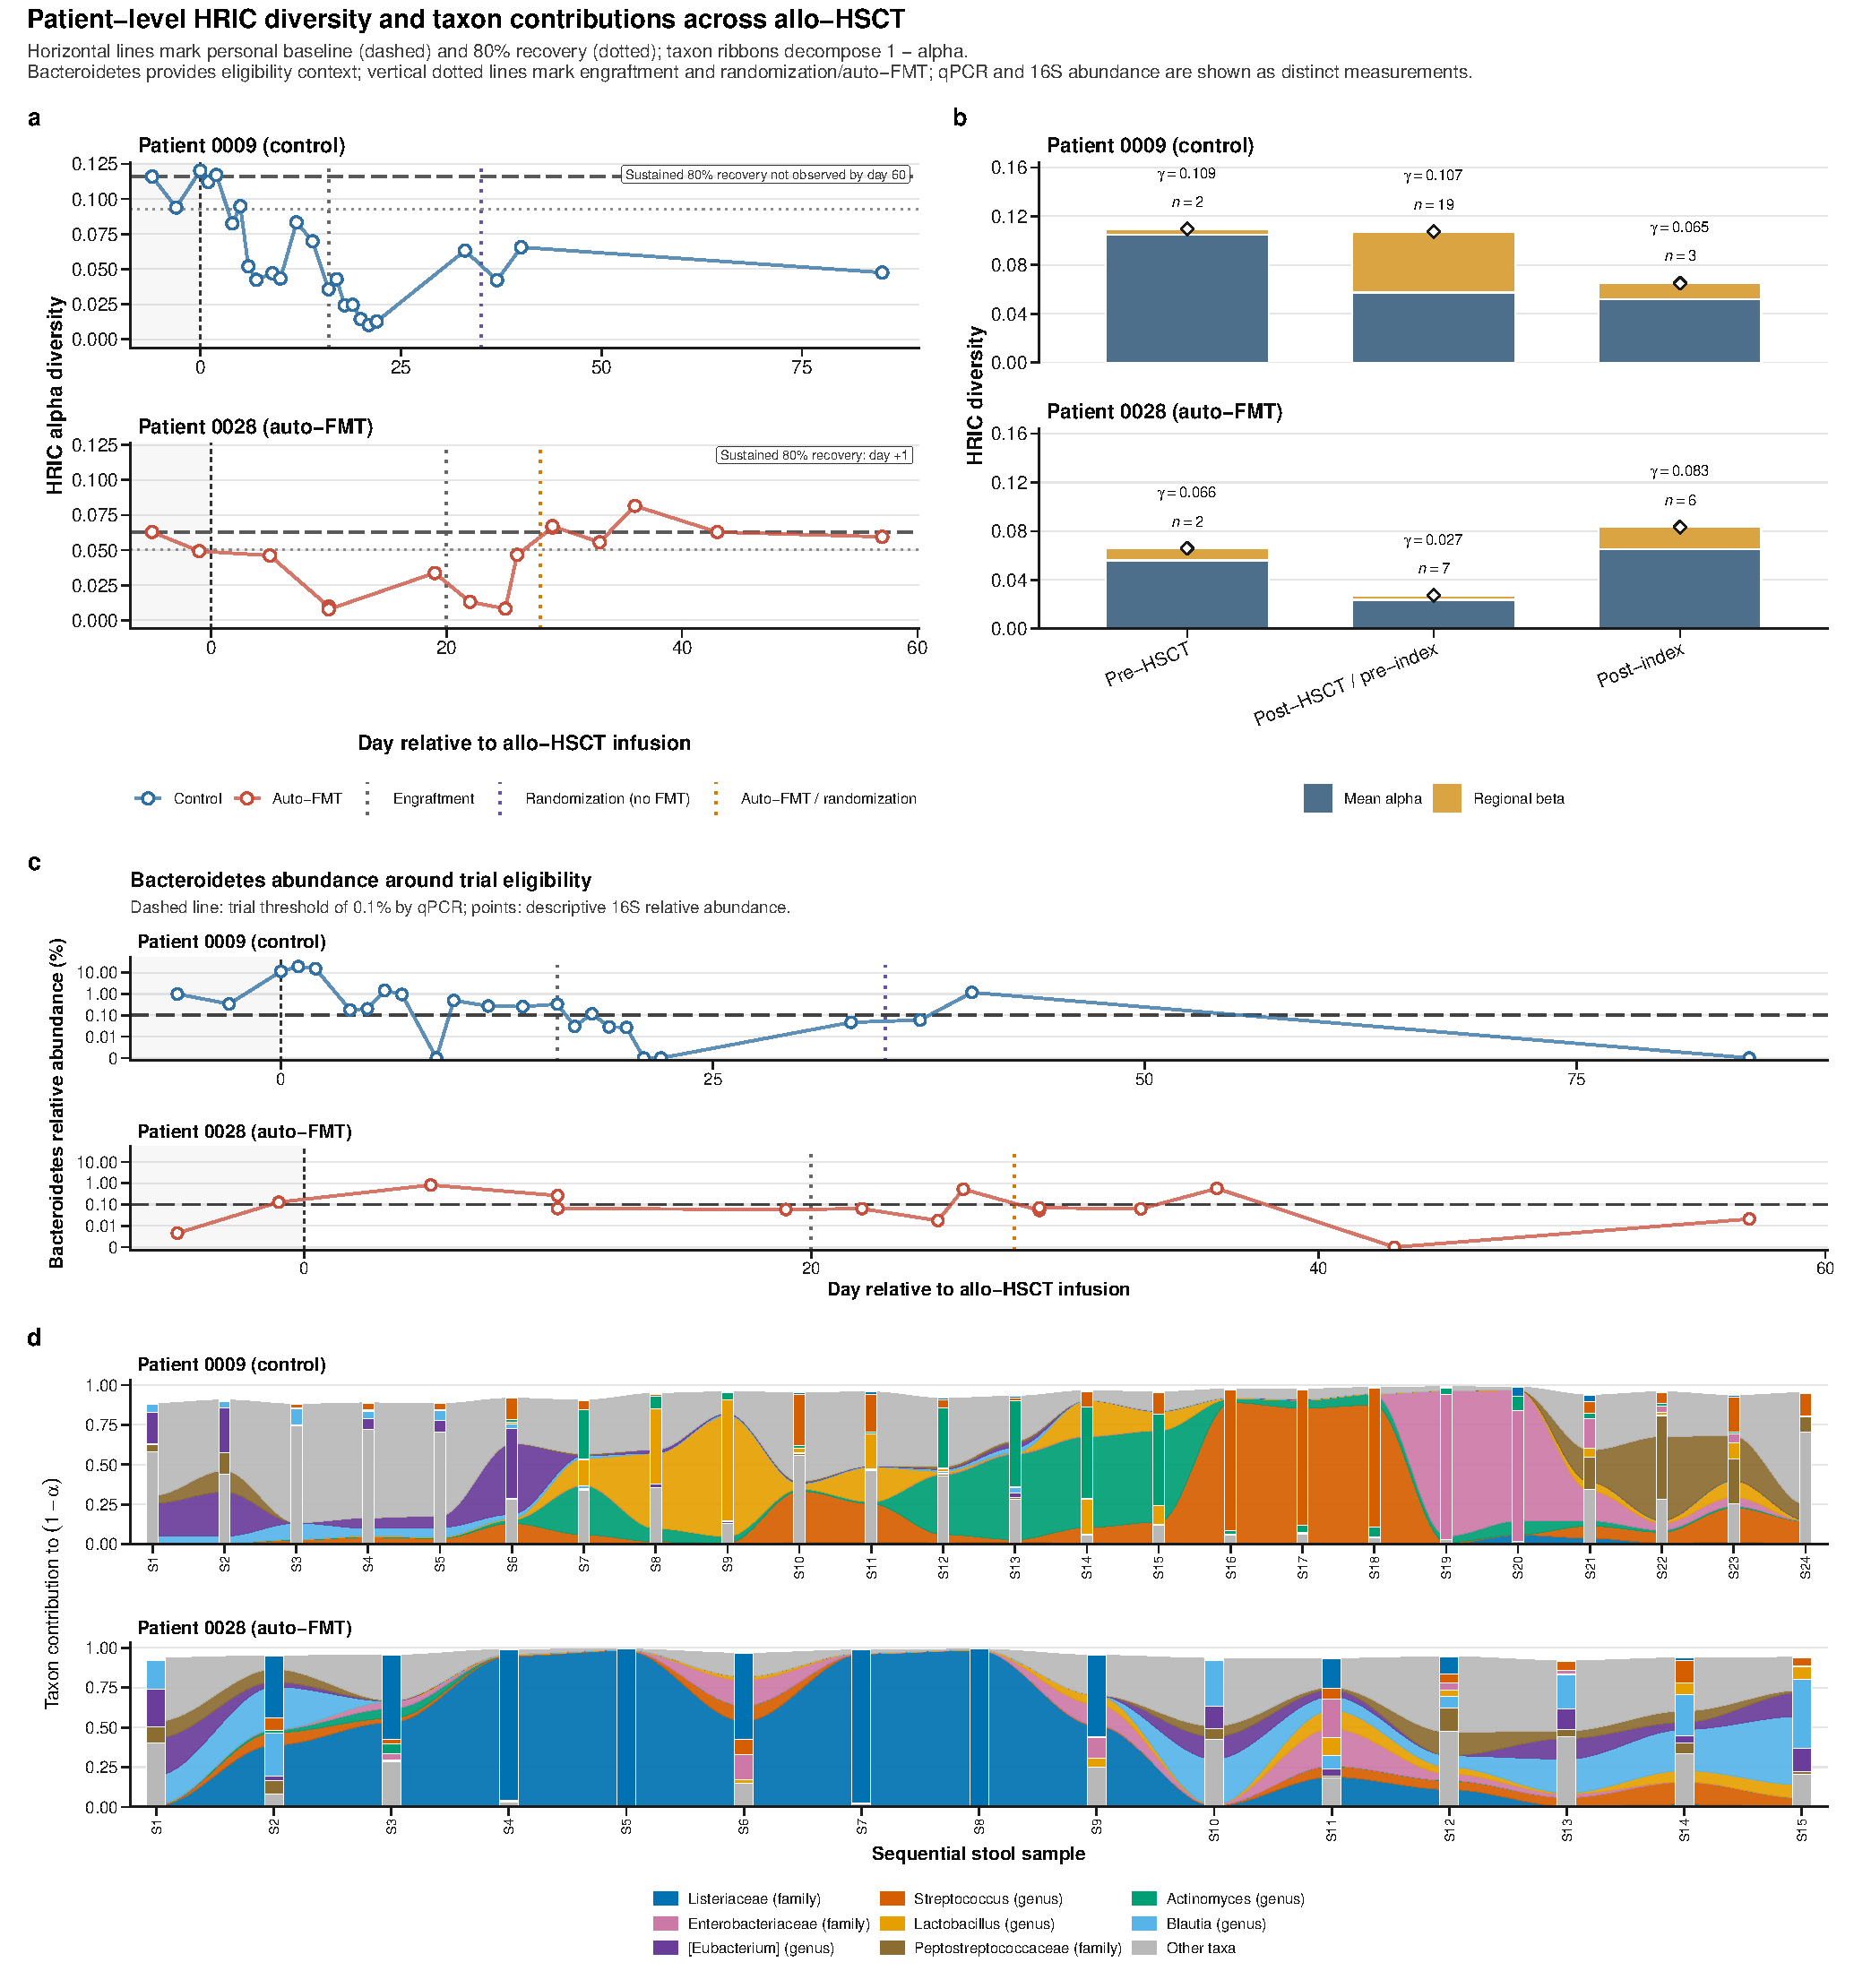
\includegraphics[
    width=\textwidth,
    height=0.58\textheight,
    keepaspectratio
  ]{figures/figure1_fmt_hric_patients_0009_0028.pdf}
  \caption{\textbf{Patient-level HRIC trajectories resolve the timing and
  taxonomic structure of microbiota recovery after allo-HSCT.}
  \textbf{a,} Longitudinal HRIC alpha diversity for patient 0009, assigned to
  control, and patient 0028, assigned to auto-FMT. Time is aligned to allo-HSCT
  infusion (day 0). Vertical dotted lines mark neutrophil engraftment and
  randomization or auto-FMT. The horizontal dashed line is the earliest
  observed pre-HSCT alpha diversity for that patient; the dotted line is 80\%
  of this value. Sustained recovery was defined descriptively as a threshold
  crossing confirmed at the next available sampling day. Patient 0028 met this
  definition at day $+1$ relative to auto-FMT, whereas patient 0009 did not
  meet it by day $+60$ relative to randomization. \textbf{b,} Within-patient
  HRIC decomposition before HSCT, after HSCT but before the index day, and
  after the index day. Bars show mean alpha diversity and beta diversity;
  diamonds show gamma diversity, with $\gamma=\bar{\alpha}+\beta$. Values of
  $n$ are stool samples. \textbf{c,} Bacteroidetes relative abundance measured
  by 16S rRNA gene sequencing. The 0.1\% line gives the trial eligibility
  threshold, which was assessed by quantitative PCR and is shown only as
  clinical context; these assays are not numerically interchangeable.
  \textbf{d,} Additive taxon contributions to the HRIC alpha deficit,
  $1-\alpha$, across sequential stool samples. The eight taxa with the largest
  aggregate contributions across the two patients are shown, with all
  remaining taxa combined as other taxa. Ribbon height represents contribution
  to the alpha deficit, not relative abundance. The two patients are
  illustrative and are not used as an estimate of the randomized treatment
  effect.}
  \label{fig:fmt-individual}
\end{figure*}

\begin{figure*}[t]
  \centering
  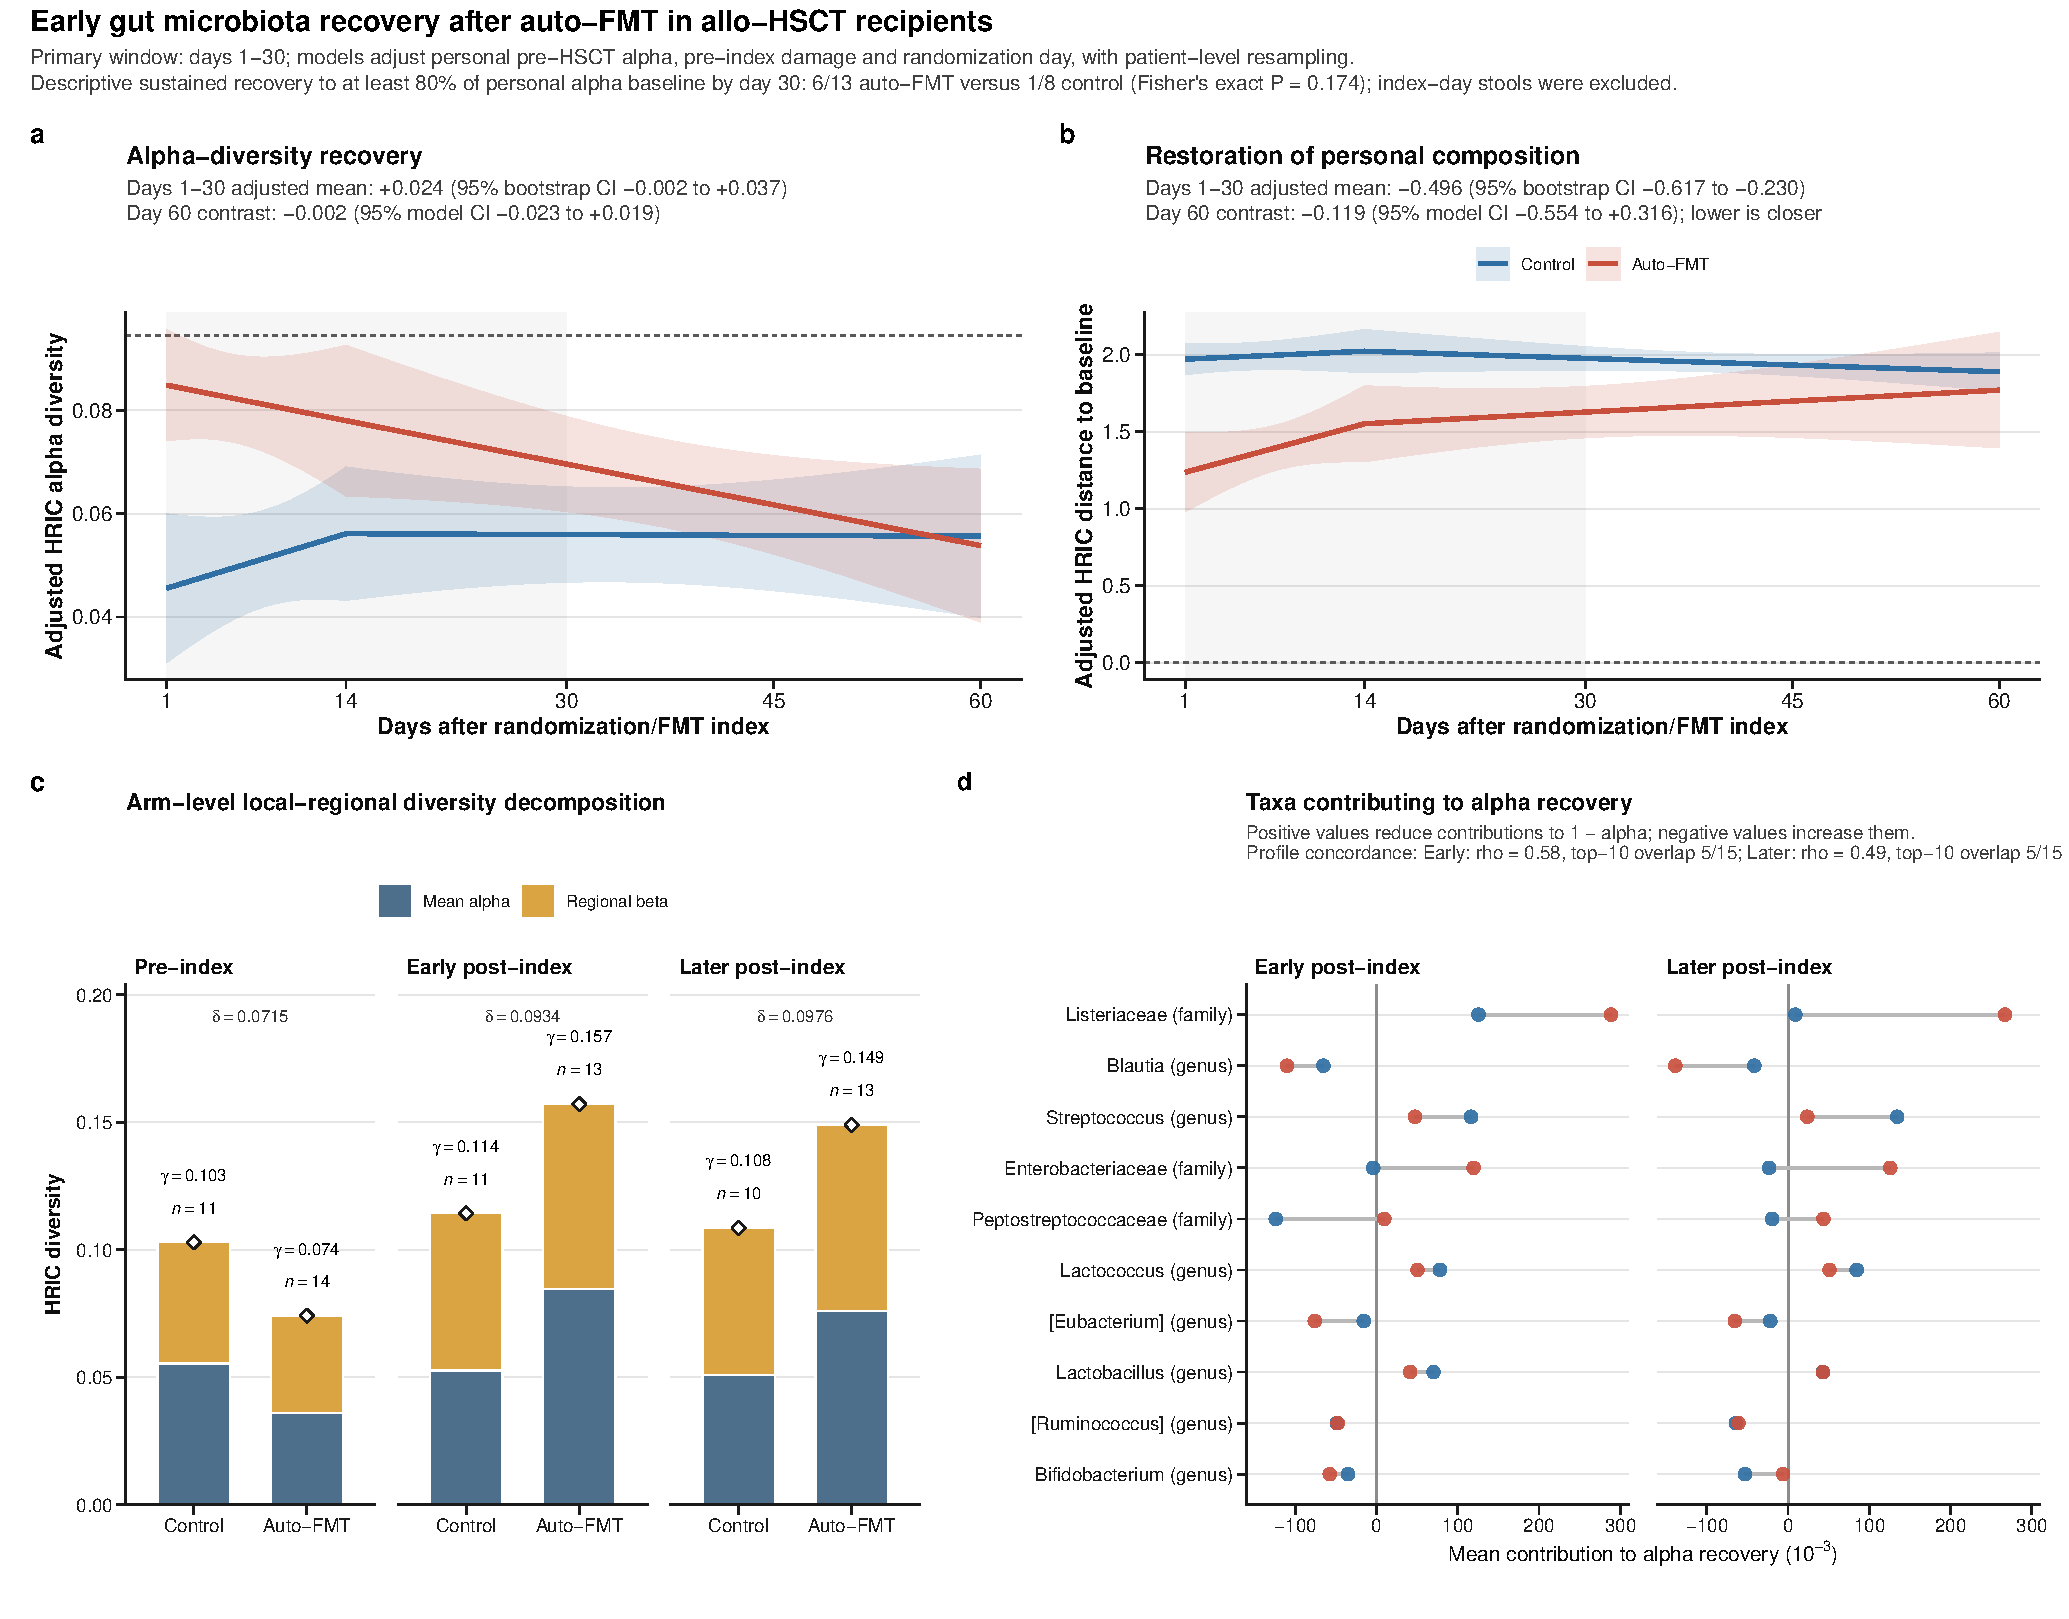
\includegraphics[
    width=\textwidth,
    height=0.53\textheight,
    keepaspectratio
  ]{figures/figure2_fmt_hric_randomized_comparison.pdf}
  \caption{\textbf{Auto-FMT is associated with earlier restoration of the gut
  microbiota in the evaluable randomized cohort.}
  \textbf{a,} Adjusted HRIC alpha-diversity trajectories during days 1--60
  after randomization or auto-FMT. The mixed-effects model included personal
  pre-HSCT alpha diversity, nearest pre-index alpha diversity, randomization
  day and a patient random intercept. The shaded region denotes days 1--30.
  The time-averaged auto-FMT minus control difference was $+0.0235$ (95\%
  stratified patient-bootstrap interval, $-0.0015$ to $+0.0373$; 4,999
  resamples). The adjusted differences were $+0.0219$ at day 14 (model-based
  95\% CI, $+0.0024$ to $+0.0414$) and $-0.0018$ at day 60 ($-0.0231$ to
  $+0.0195$). \textbf{b,} Adjusted Euclidean distance in HRIC coordinates from
  each patient's earliest pre-HSCT sample; lower values indicate greater
  restoration. The model included personal pre-HSCT alpha diversity,
  pre-index distance and randomization day, with patient-clustered uncertainty.
  The day 1--30 time-averaged difference was $-0.496$ (95\%
  patient-bootstrap interval, $-0.617$ to $-0.230$). The day-60 contrast was
  $-0.119$ (model-based 95\% CI, $-0.554$ to $+0.316$). Curves in \textbf{a}
  and \textbf{b} are fixed-effect predictions and ribbons are model-based 95\%
  confidence intervals. Index-day stools were excluded because their
  collection order relative to auto-FMT was unavailable. \textbf{c,} HRIC
  alpha-beta-gamma decomposition at the nearest stool in each prespecified
  window: pre-index (days $-28$ to $-1$), early post-index (days 1--14) and
  later post-index (days 15--60). Values of $n$ are patients; $\delta$ is the
  between-arm diversity at each landmark. \textbf{d,} Taxon-level
  contributions to alpha recovery from the pre-index landmark to the early and
  later post-index landmarks. Positive values indicate a reduction in the
  taxon's contribution to $1-\alpha$. Among taxa in the union of each arm's 50
  largest absolute contributors, recovery profiles were partly shared
  (Spearman $\rho=0.58$ early and 0.49 later). Five taxa overlapped between the
  arm-specific top-10 sets at each landmark, whose union contained 15 taxa.
  Among patients
  below 80\% of personal baseline at the index day, sustained recovery by day
  30 occurred in 6 of 13 auto-FMT recipients and 1 of 8 controls (two-sided
  Fisher's exact $P=0.174$); this threshold analysis is descriptive. The
  microbiome cohort comprised 25 evaluable randomized patients (14 auto-FMT
  and 11 control), with 98 post-index samples in the primary longitudinal
  analysis.}
  \label{fig:fmt-randomized}
\end{figure*}
